\chapter{Trigonometria}
\label{trigonometria}
\label{seniecoseni}

Come diceva il mio prof di Analisi 3, "la trigonometia serve solo a 3 categorie di persone: ai navigatori, 
agli astronomi, e agli scrittori di libri di trigonometria".
A parte la battuta, la trigonometria \'e qualcosa di molto utile nell'analisi
(meno nella vita di tutti i giorni, temo) e merita un capitolo a s\`e.

\section{Seni \& amici}

{\em Per capire questo paragrafo vi consiglio vivamente di armarvi di carta e penna e disegnare con me man mano che leggete, se no non ne uscite piu'.}

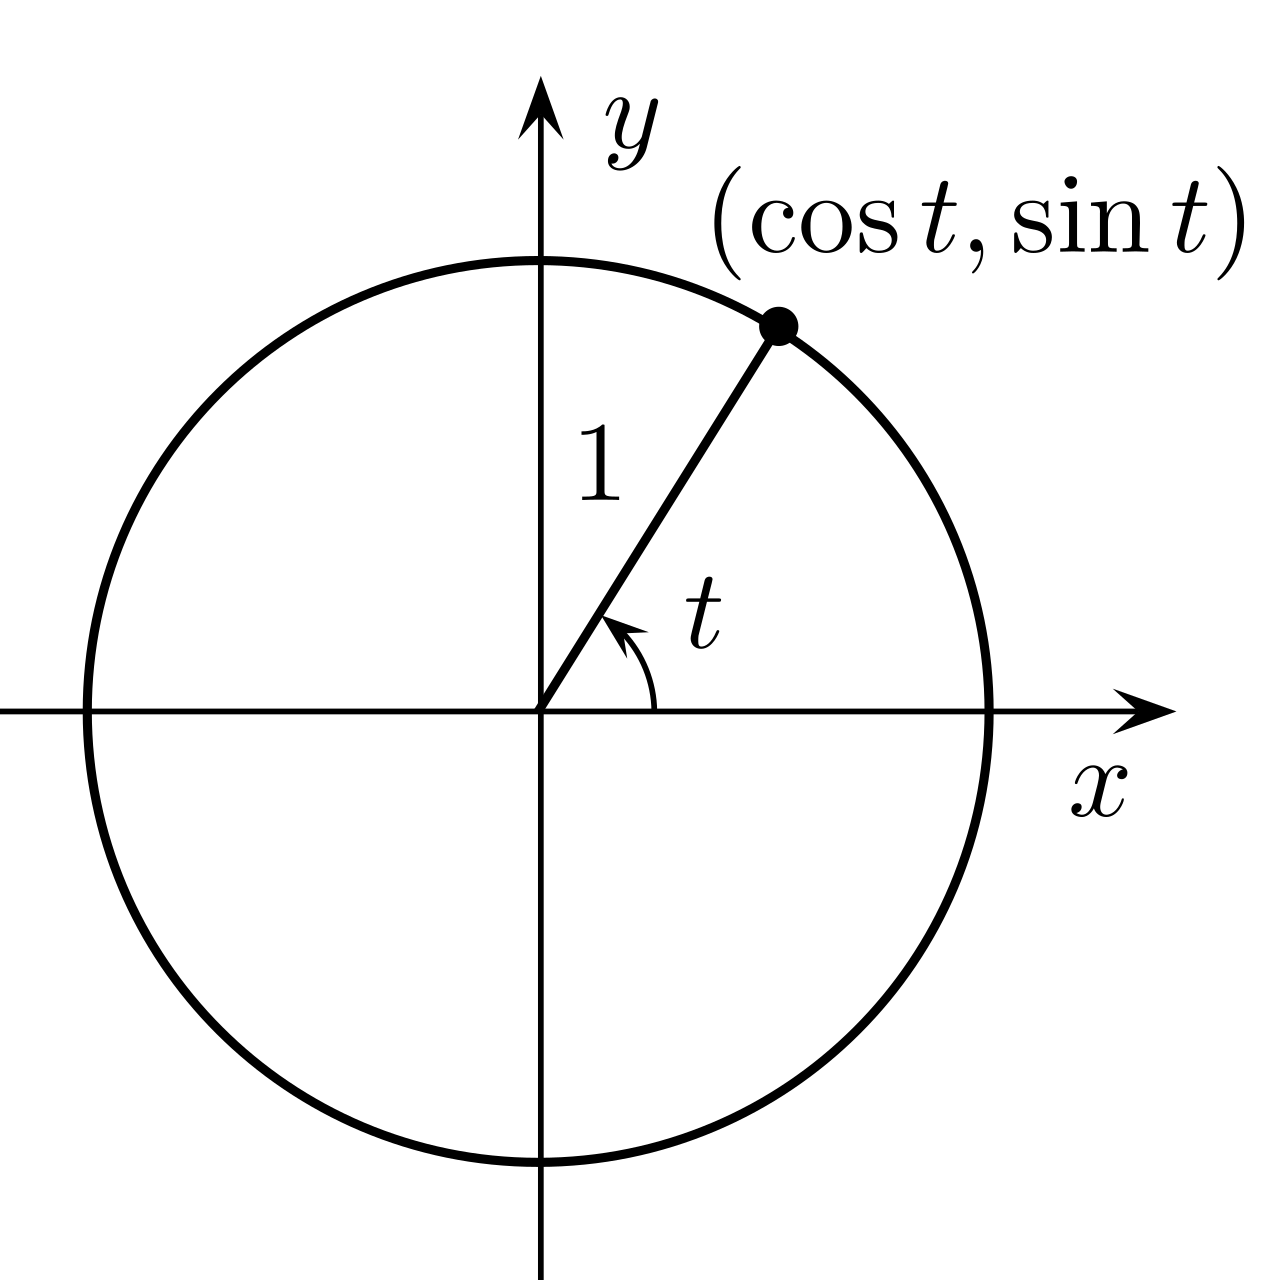
\includegraphics[height = 300pt, width = 300pt]{images/04trigonometria/circonferenza_goniometrica.png}

Il mattone fondamentale della trigonometria \'e - a mio dire - la funzione $\sin(x)$. La funzione coseno \'e molto simile alla funzione
seno (cos\'i come seni e sederi sono due caratteristiche indissolubili in una donna), e ha quindi pi\'u senso entrare nel merito della
prima per poi vedere le affinit\'a con la seconda. Prendete carta e matita e disegnate una circonferenza di raggio $1$ sugli assi cartesiani
con centro nell'origine $= \equiv (0,0)$. Se l'avete disegnata bene, osserverete che essa interseca gli assi nei punti 
$E \equiv (1,0)$, $N \equiv (0,1)$, $W \equiv (-1,0)$ (ovest), $S \equiv (0,-1)$. 

Prendete una semiretta che parte dall'origine e taglia il primo quadrante circa a met\'a, ma abbastanza bassa (in modo che l'angolo $E\stackrel{\wedge}{O}P$ sia di circa 30 gradi). 
Chiameremo $\theta$ l'angolo tra la semiretta per $\overrightarrow{OP}$ e la semiretta per $\overrightarrow{OE}$. La funzioen seno \'e definita
come l'altezza del punto P al variare dell'angolo $\theta$ (e il coseno ne \'e l'ascissa, ovvero la proiezione orizzontale).
Segue direttamente dalla definizione che il punto P, al variare di $\theta$, varr\'a: $P \equiv (\cos(\theta),\sin(\theta))$.
L'angolo $\theta$ (e qui davvero non chiedetemi il perch\'e\footnote{OK, se insistete vi dico la mia teoria: i numeri complessi
sul piano cartesiano hanno il numero pi\'u importante (uno) corrispondente alla coppia [1,0] che si trova appunto a EST.})
viene posto a zero nel punto $E$, e si muove in senso antiorario (anche qui ho una mia teoria sul perch\'e).

Non credete mi sia dimenticato di voi, prendete carta e matita e disegnate i tre punti notevoli che vi dir\'o: tagliate il primo quadrante
in due parti uguali (quindi $\theta$ vale $45$) e intersecatelo con la circonferenza goniometrica (ovvero una circonferenza di raggio uno centrata nell'origine).
Tagliatelo ora in 3 parti uguali, tagliando sempre il quadrante di nordest con angoli di $30$ e $60$. I tre punti in cui la circonferenza taglia la bisettrice
e le due 'trisettrici' li chiameremo $A,B,C$ partendo da est e arrivando a nord. Dalla definizione di $\theta$ che vi ho dato, gli angoli relativi ai tre punti
sono, rispettivamente, $30,45,60$. Dato che le cose son troppo facili, vi devo dire che i matematici non ragionano in gradi. L'angolo {\em naturale} che
si usa (e con ottime ragioni) \'e il radiante, che vale $\frac{180}{\pi}$ (circa $57,3$). Se pensate che $180$ sian $3,14$ radianti non vi passer\'a mai,
quindi vi do un consiglio: dimenticate la parola radiante e fate finta che l'angolo si misuri in 'pigrechi': un angolo giro son due pigrechi, un angolo retto
\'e mezzo 'pigreco', e un angolo piatto \'e un pigreco esatto (to', che coincidenza). Cosa ulteriore, all'occorrenza un 'pigreco' vale {\em esattamente}
quanto il $\pi$ che avete conosciuto alle medie; ma per ora dimenticatevene, fate finta che sia un'altra cosa. Se proprio non vi piace come atteggiamento,
chiamate $\pi$ radianti 'un gradone'; e adottate come suo simbolo $\pi$: cos\'i vi ho fregati di nuovo. Attenti, met\'a degli errori che si fanno con
la trigonometria nascono da quanto poco sia intuibile un radiante, quindi perdeteci qualche minuto...

Adesso prendete $E,A,B,C,N$ e calcolatemi i valori delle $x$ e delle $y$. E' molto facile, perci\'o calcolatevelo e imparatevi a memoria questi valori.
Nel disegno che segue ho messo A,B,C nel terzo quadrante invece che nel primo per non deturpare il generico seno e coseno (e uso X come angolo invece di
theta per problemi grafici). Notate le due trisettrici in viola e la bisettrice in arancione.

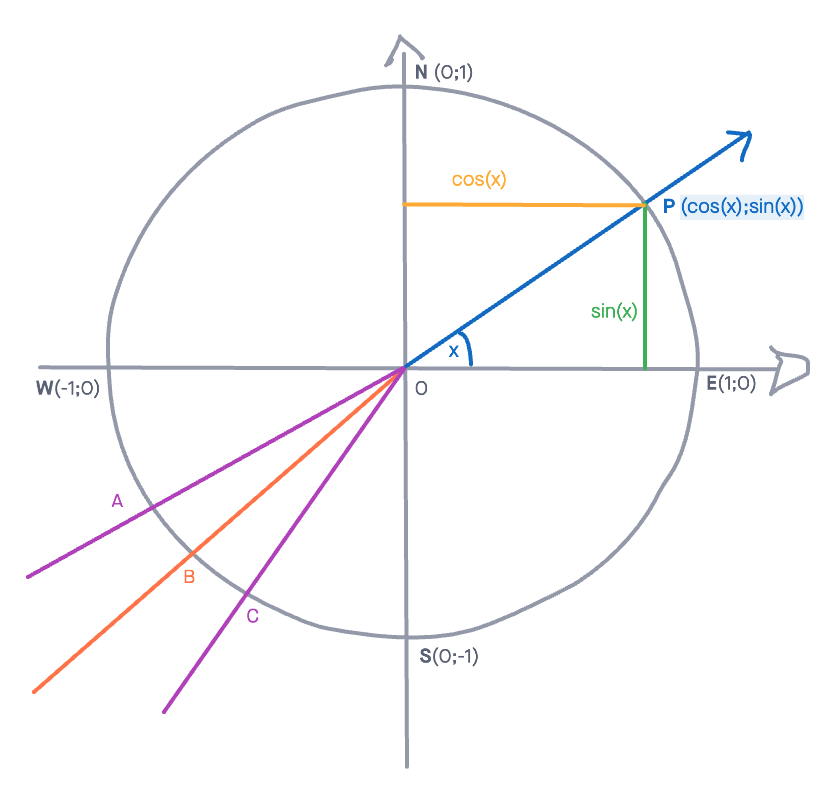
\includegraphics[height = 300pt, width = 300pt]{images/04trigonometria/circonferenza goniometrica con A B C.png}


Allora, vi aiuto: $E$ e $N$ sono dati dall'inizio; $BOE$ \'e un bel triangolo rettangolo isoscele; ne conoscete l'ipotenusa ma non i cateti (la cui
lunghezza poniamo uguale a $x$). Come calcolarlo? Usiamo pitagora, sapendo che l'ipotenusa \'e unitario: 
$x^2+x^2=1^2 \longrightarrow x=\frac{\sqrt{2}}{2}\simeq 0.707$. Ora veniamo ad $A$: $OAA'$ (con $A'$ proiezione di $A$ sul lato di sud est
della circonferenza) \'e un triangolo equilatero, lo si vede dagli angoli. Ma allora, l'ipotenusa \'e noto, l'altezza di $AA'$ \'e sempre unitaria,
manca solo l'ascissa di $A$ che \'e l'altezza dl triangolo equilatero. Si ricava che $y_A=\frac{1}{2}$ (poich\'e \'e met\'a di $AA'$) e con pitagora
possiamo anche scoprire $x_A: x^2+(\frac{1}{2})^2=1^2 \longrightarrow x_A=\frac{\sqrt{3}}{2} \simeq 0.866$ (il famoso apotema del triangolo, pensa che
coincidenza!). Mettendo insieme i valori, otteniamo che:

\begin{equazione}
	E \equiv (1;0); \theta=0 \\
	A \equiv (\frac{\sqrt{3}}{2};\frac{1}{2}); \theta=\frac{\pi}{6} \\
	B \equiv (\frac{\sqrt{2}}{2};\frac{\sqrt{2}}{2}) 			\theta=\frac{\pi}{4} \\
	C \equiv (\frac{1}{2};\frac{\sqrt{3}}{2}) \theta=\frac{\pi}{3} \\
	N \equiv (0;1) \theta=\frac{\pi}{2} \\
\end{equazione}

Negli altri quattro quadranti i valori sono gli stessi, solo che cambiano i segni (nella met\'a sud il seno \'e negativo, nella met\'a ovest il coseno \'e negativo).
Ci sono molte cose da notare: vediamone alcune. Anzitutto, seno e coseno si scambiano al passare dei $\ang{45}$: i valori a $\ang{30}$ sono gli stessi di $\ang{60}$ e state tranquilli
che lo stesso vale anche tra $\ang{20}$ e $\ang{70}$ (sebbene sian valori un po' pi\'u ostici da calcolare); ehi, ma se questa propriet\'a \'e vera, seno e coseno devono
essere per forza uguali in $\ang{45}$! E infatti \'e cos\'i \footnote{Riflettete su questa cosa, se avete un minuto.}! Altra cosa: gli angoli in natura sono piccoli
(ho fatto molti studi psicologici alla Peter Vienkmann e vi posso assicurare che se chiedete a qualcuno di disegnari un angolo questo sar\'a dannatamente vicino a $30$);
se \'e vero che nella vostra vita avete in mente angoli piccoli, avete in mente coseni molto grandi (tra $0,8 e 0.9$) e seni piccoli (tra $0.3 e 0.5$). Questo discorso {\em \'e}
effettivamente da pazzi, ma vi aiuter\'a (spero) quando vi troverete a confondervi tra seni e coseni all'esame. Ricordate: per angoli piccoli il coseno \'e tanto e il seno \'e
piccolo; e di solito \'e il seno che pi\'u si avvicina alla met\'a ed \'e il pi\'u sensibile alle variazioni (ovvero se variate di poco l'angolo, il seno varier\'a di pi\'u
in proporzione\footnote{Poich\'e a mio parere questa regola potrebbe salvarvi ad un esame di Analisi o soprattutto di Meccanica Razionale, vorrei darvi una regola per ricordarvela
a vita: {\bf "Se vedete una donna con il seno piccolo e il sedere (= coseno) grosso, vi girerete poco per guardarla (= angoli piccoli)"}. L'esempio \'e terribile, lo so,
ma ho visto troppi amici cadere per un errore di segno o di angolo in trigonometria, quindi mandatelo a mente, o trovate un esempio migliore e pi\'u gender-neutral (faccio
fatica a visualizzare seni per uomini)}.

Per quanto riguarda i segni, ricordate che il seno \'e negativo per angoli che vanno da $\ang{180}$ a $\ang{360}$, 
mentre i coseni son negativi da $\ang{90}$ a $\ang{270}$\footnote{Anche qui, regola mnemonica (e non importa che 
sia vera o meno): {\bf "Le scandinave (=nord) hanno un bel seno, e le russe (=est) hanno un bel sedere" (chido scusa per il sessismo della frase, 
vi chiederei di aiutarmi con un esempio mnemonico che sia piu' inclusivo)}.}.

Ecco qui di sotto alcuni valori notevoli su tutta la circonferenza goniometrica: come vedete sono tutti speculari a meno del segno nei quadranti
dopo il primo.

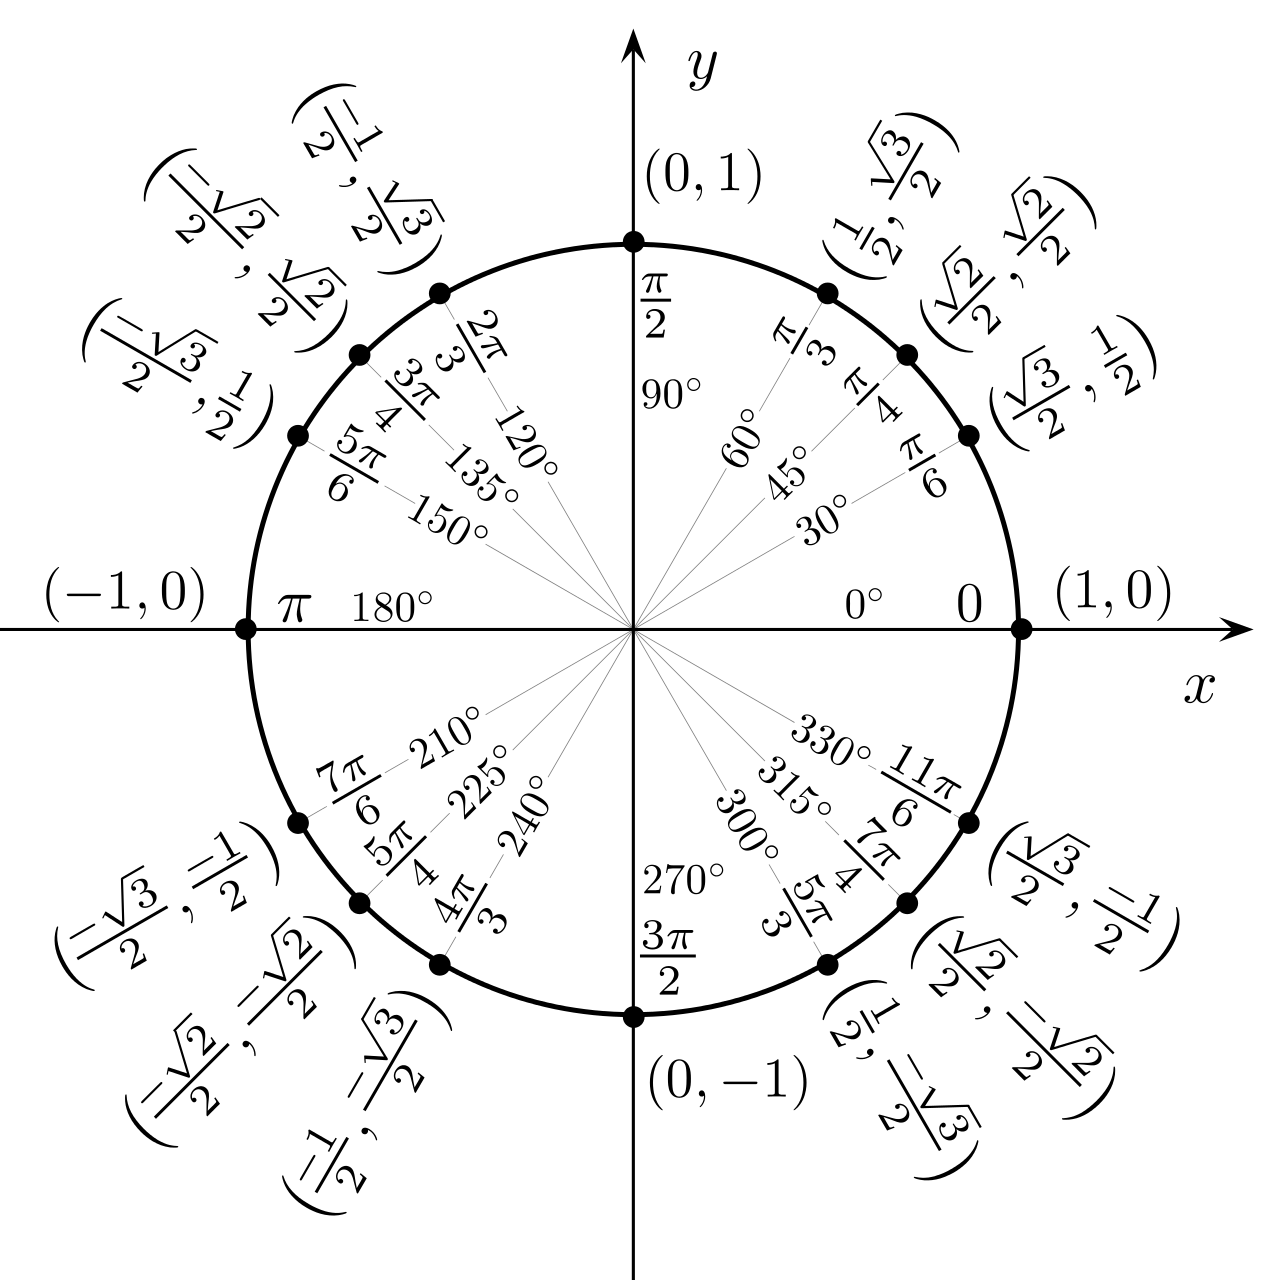
\includegraphics[height = 300pt, width = 300pt]{images/04trigonometria/seni_coseni_per_angolo.png}

Ricordate che il $90\%$ degli errori nella trigonometria sono nei segni o nella confusione tra seno e coseno, mentre il $999\%$ rimanente sta negli errori di scrittura. :)

\begin{esercizio}
Quanto vale circa il seno di $\ang{40}$? E il seno di $40$? Non dico di dirmi i valori esatti, ma a occhio? Riuscite ad abbozzare un valore senza calcolatrice
e poi vedere se avete sbagliato di molto? Lo zio Ric vi consiglia di perderci qualche minuto, \'e {\em davvero} istruttivo. Scrivete su un pezzo di carta
la vostra soluzione \em{prima} di usare la calcolatrice. \emph{Hey tu! Ti ho visto, stai barando! Via il telefonino!}
\end{esercizio}


\section{Altre funzioni trigonometriche}

Ci sono altre funzioni trigonometriche; le pi\'u famose sono la tangente ($\doteq \sin(x)/\cos(x)$),
la secante ($\frac{1}{\cos(x)}$) e la cosecante ($\frac{1}{\sin(x)}$). in tanti anni non ho mai trovato alcuna applicazione
pratica a secanti e cosecanti, quindi non m'impegner\'o a trovare qualche rilevanza.
La tangente, invece \'e importantissima e sarebbe opportuno studiarla un po'. Essa \'e periodica di periodo $\pi$, e
tende all'infinito nei suoi estremi pi\'u famosi ($\pm \pi/2$). Se v'interessa, la sua funzione inversa (l'arcotangente)
\'e una delle mie funzioni preferite e si usa abbastanza nell'elettronica (insieme al logaritmo, e' una delle due funzioni trascendenti con derivata algebrica).
Credo sia la funzione pi\'u educata seppur elegante che io conosca.
